\subsection{Statistiske ytelsesindekser}
Det nevnes tre bruksområder for indekser som måler statistisk ytelse
\begin{itemize}
\item Regresjonsproblemer
\item Klassifiseringsproblemer
\item Sammenligning av sannsynlighetsfordelinger
\end{itemize}
Vi går gjennom disse i den rekkefølgen.

\subsubsection{Regresjonsproblemer}
En naturlig indeks er \textbf{Mean Squared Error (MSE)}
\begin{equation}
\textrm{MSE} = \mathbb{E}\left[\|\theta-\widehat{\theta}\|^{2}\right]
\end{equation}

Av denne følger \textbf{Root Mean Square Error}
\begin{equation}
\textrm{RMSE} = \sqrt{\mathbb{E}\left[\|\theta-\widehat{\theta}\|^{2}\right]}
\end{equation}

Det er viktig å merke seg at siden MSE er en funksjon av $\theta$, så kan den ikke regnes ut. Hvorfor bryr vi oss om den da? Tja, den kan i hvert fall inspirere lignende indekser. \textbf{Residual Sum of Squares (RSS)} baserer seg på residualene til estimatene
\begin{equation}
\operatorname{RSS}(\widehat{\theta}):=\sum_{i}\left(y_{i}-\widehat{y}_{i}(\widehat{\theta})\right)^{2}
\end{equation}

Det finnes imidlertid problemer med alle disse. Først og fremst er det et problem at de er avhengig av mengden av og størrelsen på dataen man vurderer estimatene av. Man vektlegger å unngå avvik i estimatene fra store målinger mer enn små. En metode som fungerer noe bedre, uten å bruke normalisering, er å bruke 1-normen i stedet for kvadratet. Dette gjøres i \textbf{Mean Absolute Deviaton (MAD)}
\begin{equation}
\mathrm{MAD}:=\mathbb{E}[|y-\widehat{y}|]
\end{equation}

En metode som bruker en form for normalisering er \textbf{Fraction of Variance Unexplained (FVU)}
\begin{equation}
\mathrm{FVU}(\widehat{\theta}):=\frac{\operatorname{RSS}(\widehat{\theta})}{\operatorname{var}(y)}=\frac{\sum_{i}\left(y_{i}-\widehat{y}_{i}(\widehat{\theta})\right)^{2}}{\sum_{i}\left(y_{i}-\frac{1}{N} \sum_{i} y_{i}\right)^{2}}
\end{equation}
Denne må tolkes med måte, siden hva som er en god forklaringgrad er veldig avhengig av hva slags felt man jobber i, og det konkrete bruksområdet. Dette er uansett en mye brukt indeks, men da i form av $R^{2}$
Denne tolkes som "andel av variansen i avhengig variable som er predikerbar fra de uavhengige variablene".

\subsubsection{Klassifiseringsproblemer}
Vi diskuterer her klassifisering i form av "ja/nei". Da kan man gjøre to typer feil: Falsk positiv (\textbf{Type 1}) og falsk negativ (\textbf{Type 2}). Figur \ref{fig:klassifisering} viser definisjonen på en del uttrykk som beskriver egenskapene til en klassifikator.

\begin{figure}[h]
\centering
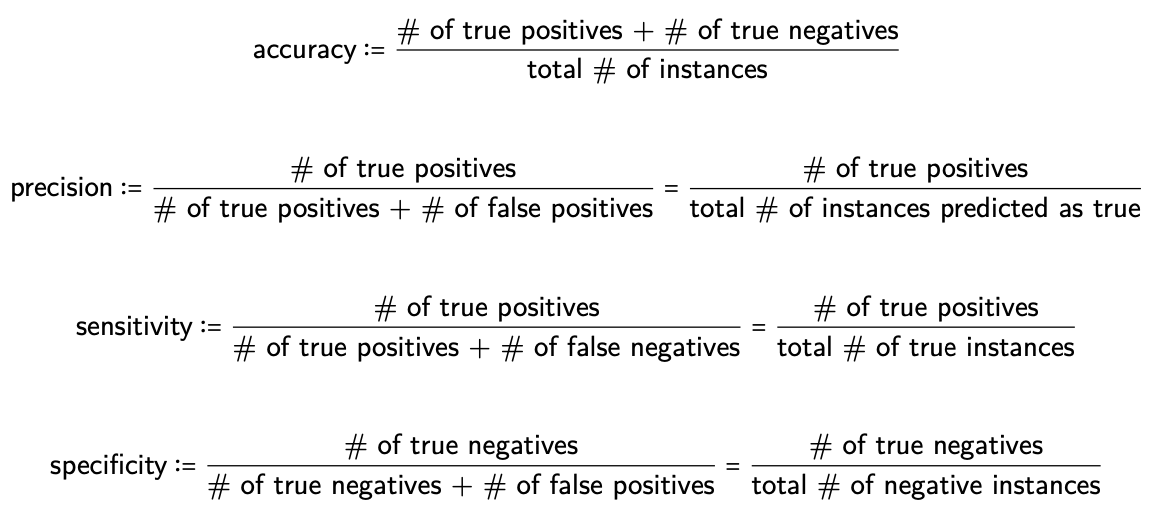
\includegraphics[width=0.8\textwidth]{Figurer/klassifisering.png}
\caption{Egenskaper til klassifikator}
\label{fig:klassifisering}
\end{figure}

Muntlig kan disse forklares som
\begin{itemize}
\item \textbf{Prevalens} -- Hvor ofte opptrer ja-tilfellet i datasettet vårt?
\item \textbf{Nøyaktighet} -- Hvor ofte har klassifikatoren rett?
\item \textbf{Feilklassifiseringsrate} -- Hvor ofte tar klassifikatoren feil?
\item \textbf{Presisjon} -- Når klassifikatoren gjetter ja, hvor ofte er dette rett?
\item \textbf{Falsk positiv-rate} -- Når svaret er nei, hvor ofte gjetter klassifikatoren ja?
\item \textbf{Sensitivitet} -- Når svaret er ja, hvor ofte gjetter klassifikatoren ja?
\item \textbf{Spesifitet} -- Når svaret er nei, hvor ofter gjetter klassifikatoren nei?
\end{itemize}

Man kan også kombinere to av disse for å få \textbf{F1-score}
\begin{equation}
\textrm{F1-score} = 2 \frac{\textrm{presisjon} \cdot \textrm{
sensitivitet}}{\textrm{presisjon} + \textrm{
sensitivitet}}
\end{equation}

Om man vil finne ut hvor ulike to klassifikatorer er, kan man bruke \textbf{Kappa-koeffisient}. Dette forklares ikke mer, men det eksisterer.

\subsubsection{Sammenligning av sannsynlighetsfordelinger}
Her kan man bruke \textbf{Kullback-Leibler-divergens}.